% !TEX root = memoire/main.tex
\chapter{Développement de méthodes permettant l'adaptation du filtre de Kalman d'ensemble avec des simulations sans maillage}

---------------
\section{Objectifs}
Le filtre de Kalman présenté en Section~\ref*{sec:enkf} est un filtre séquentiel adéquat pour appliquer des méthodes d'assimilation pour des modèles de grande dimension et non-linéaire. Il consiste à mettre à jour un ensemble d'état en déterminant un gain de Kalman pour combiner l'état prédit et un terme d'innovation fonction de l'erreur de prédiction. Lorsque l'état est défini à l'aide d'une discrétisation eulérienne, la mise à jour du filtre peut être facilement. Il en est de même pour les états défini sur une

%
% Revoir introduction article.
%

En particulier ce gain va dépendre des statistiques de l'état

Toutefois, la mise à jour du filtre de Kalman d'Ensemble est dépendante de la discrétisation de l'état de ses membres pour le calcul du gain de Kalman d'ensemble. De plus, la mise à jour du filtre de Kalman d'Ensemble est basé sur une combinaison linéaire des membres au travers du gain de Kalman d'ensemble, celle-ci entraîne une explosion du nombre de particules dans la définition de la solution analysée.

L'objectif de ce chapitre est donc de présenter un certain nombre d'adaptation du filtre de Kalman d'Ensemble qui puisse être appliquées à des simulations sans maillage.

Pour cela, nous reformulons tout d'abord l'expression de la mise à jour afin qu'elle soit indépendante de la définition de l'état.
Enfin, les solutions analysées étant des combinaisons linéaires des particules de l'ensemble des membres, nous proposons de développer des méthodes pour réduire l'augmentation exponentielle des particules.

\section{Mise à jour défini dans l'espace des membres}~\label{sec:enkf_membre}

La mise à jour du filtre de Kalman se base sur l'approximation des statistiques des distributions de l'état et des observations pour approché le gain de Kalman (voir \eqref{eq:enkf_formula}).

Dans le cas d'un état qui repose sur une discrétisation particulaire, on ne peut directement évaluer ses statistiques directement sur les quantités particulaires, c'est à dire positions et intensité. En effet, chaque membre possède


Heureusement La particularité du filtre de Kalman d'ensemble est qu'il fait une approximation de faible rang du gain de Kalman. Nous avons montré en Section~\ref{sec:faible_rang} que la mise à jour s'exprimait comme une combinaison des états de l'ensemble $X$.

De cette manière la mise à jour est déterminé comme

\begin{equation*}
    \mstate_a = \mstate_f + \mstate_f \Fcorr, \quad \Fcorr = \frac{1}{\sqrt{N-1}} \annomY_f^T {(\annomY_f \annomY_f^T + \bm R)}^{-1}(\mdata - \mpred).
\end{equation*}.

Où la matrice de correction $\Fcorr \in \mathbb{R}^{N\times N}$ est indépendante de la discrétisation.

De plus, en utilisant la formule de Sherman-Morrison-Woodbury (SMW)~\cite{SMW}, la matrice peut être calculé à l'aide uniquement de l'inversion de la matrice $\bm R$ et d'une matrice de taille $N$

\begin{equation*}
    \Fcorr = \frac{1}{\sqrt{N - 1}} {(\bm I_N + \annomY_f^T\bm R^{-1}\annomY_f)}^{-1}\annomY_f^T \bm R^{-1} (\mdata - \mpred),
\end{equation*}ce qui devient avantageux dans le cas où $\bm R$ est une matrice diagonale et $N < N_{\text{obs}}$.

Cette indépendance est possible par la linéarisation de l'opérateur d'observation et l'approche par rang faible. D'autres versions du filtre EnKF offre les mêmes propriétés. C'est le cas du \textit{ensemble transform Kalman filter} (ETKF, \cite{Hunt2007}). En effet, ce filtres travaillent directement dans l'espace de perturbation.

Travailler dans l'espace de perturbation des observations $\bm Y^T$ permet d'éviter d'exprimer les statistiques de l'état.

L'étape d'analyse est donc une combinaison qui ne dépend que des observations $\bm y$ (perturbé pour le filtre stochastique), les prédictions de l'ensemble $\left[\mathcal{H}(x^i_f)\right]_{i=1}^{N}$, et la matrice de covariance d'erreur $R^{1}$. De cette manière, pour chaque membre $i$, le champ analysé $\fstate_i^a$ peut être déterminé en tout point de l'espace $\bm x \in \omega$ grâce aux champs prédits $\fstate_j^f$ tel que

\begin{equation}
    \fstate_i^a(\bx) =\fstate_i^f(\bx) + \sum_{j=1}^{N} F_{ji} \fstate_j ^f(\bx), \quad i = 1, \dots, N.
\end{equation}

\section{Mise à jour comme solution particulaire}

Les solutions analysées peuvent être décomposées à partir de la discrétisation particulaire des champs $\fstate_i^f$.

Dans un premier temps, nous supposons que les positions de particules sont les mêmes pour tous les membres. On note $(\bx_1,...\bx_{N_p}) \in \mathbb{R}^d$ les positions des centres de particule, deux à deux distincts de telle sorte que, pour tout $\bx \in \mathbb{R}^d$

\begin{eqnarray*}~\label{eq:enkf_formula_same_part}
    \fstate_i^a(\bx) &=& \fstate_i^f(\bx) + \sum_{j=1}^{N} F_{ji} \fstate_j ^f(\bx) \\
    &=& \sum_{p=1}^{N_p} \Gamma^f_{p,i} \phi_{\varepsilon}(\bx - \bx_p) + \sum_{j=1}^{N} F_{ji} \sum_{p=1}^{N_p} \Gamma_j ^f(\bx) \phi_{\varepsilon}(\bx - \bx_p) \\
    &=& \sum_{p=1}^{N_p} \left[\Gamma^f_{p,i} + \sum_{j=1}^{N} F_{ji} \Gamma^f_{p,j} \right] \phi_{\varepsilon}(\bx - \bx_p).
\end{eqnarray*}

En utilisant la linéarité de la décomposition par rapport aux intensités $\Gamma^f_{p}$, l'analyse pour chaque membre peut directement s'exprimer pour chaque membre en appliquant la mise à jour directement sur les intensités. En notant $\bm \Gamma$ la matrice dont la i-ème colonne est $(\Gamma_{1, i},...\Gamma_{N_p, i})$, la mise à jour est directement exprimé comme

\begin{equation*}
    \bm \Gamma^a = \bm \Gamma + \bm \Gamma \Fcorr.
\end{equation*}

Cependant, dans le cas général les positions de particules diffèrent d'un membre à l'autre. Dans ce cas, en utilisant la décomposition particulaire des champs prédit $\mP_i^f$, la solution analysée va s'exprime comme

\begin{eqnarray*}
    \fstate_i^a(\bx) &=& \sum_{p \in \mP_i^f}\Gamma^f_p \phi_{\varepsilon}(\bx - \bx_p) + \sum_{j=1}^{N} F_{ji}  \sum_{p' \in \mP_j^f}\Gamma^f_{p'} \phi_{\varepsilon}(\bx - \bx_{p'}) \\
    &=& \sum_{p \in \mP_i^f}\left[(1 + F_{ii})\Gamma^f_p \phi_{\varepsilon}(\bx - \bx_{p})\right]   + \sum_{j\neq i} F_{ji} \Gamma^f_{p'} \phi_{\varepsilon}(\bx - \bx_{p'}) \\
    &=& \sum_{j=1}^{N} \sum_{p \in \mP_j^f} \Gamma^a_p \phi_{\varepsilon}(\bx - \bx_p).
\end{eqnarray*}
$\fstate_i^a$ est bien une solution particulaire.


Sans perte de généralité, en supposant que chaque particules ont des positions $x_p$ distincts, alors l'espace d'approximation est de dimension $\sum_{i=1}^{N} \text{Card}(\mathcal{P}^f_i)$.

Ainsi, à chaque étape d'assimilation de données, le nombre de particule pour approcher la solution analysée augmente exponentiellement avec l'union des particules de tous les membres comme en Figure~\ref{fig:support_particles}.

\begin{figure}~\label{fig:support_particles}
    \centering
    \begin{subfigure}{0.5\textwidth}
        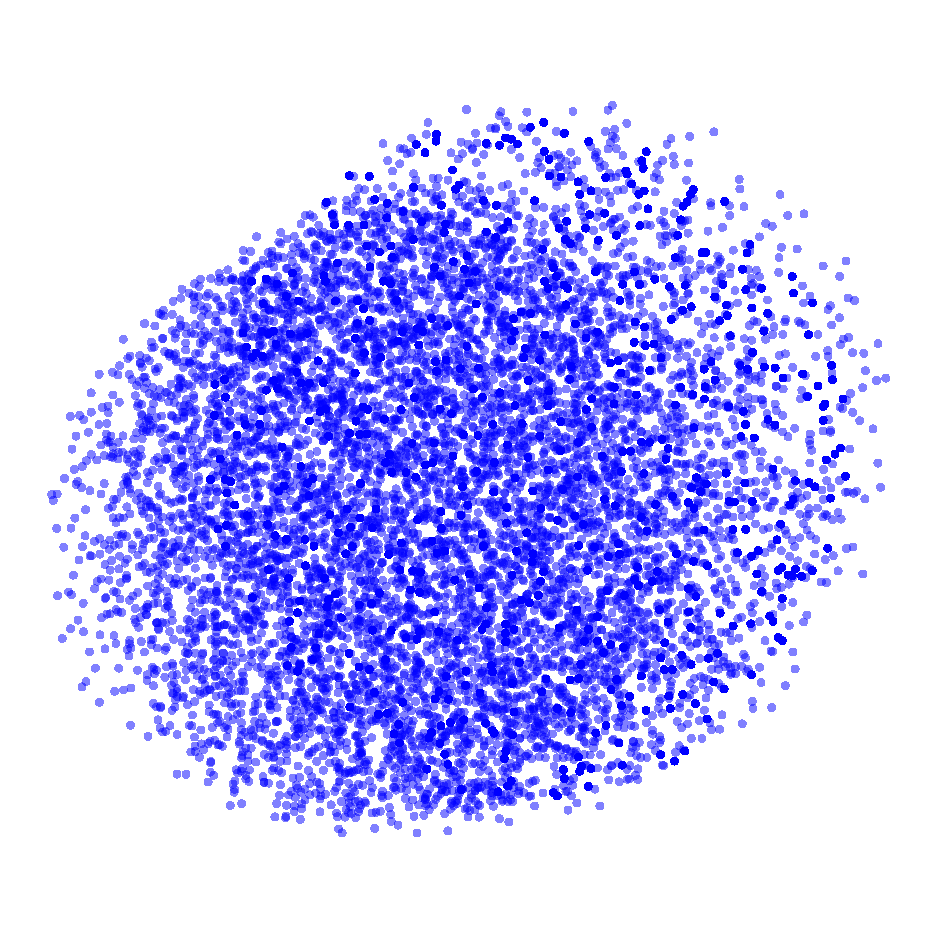
\includegraphics[width=\textwidth]{images/all_particles.pdf}
    \end{subfigure}
    \begin{subfigure}{0.5\textwidth}
        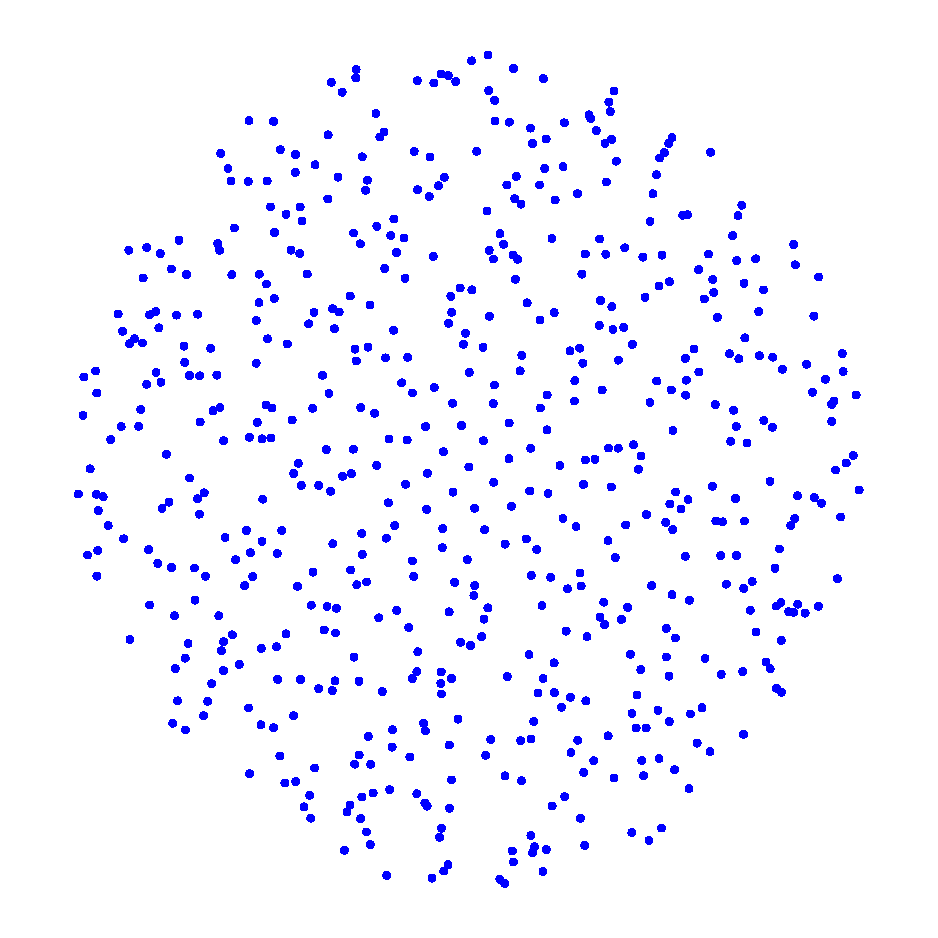
\includegraphics[width=0.5\textwidth]{images/memb_particles.pdf}
    \end{subfigure}
    \caption{Support de particule d'un membre avant et après correction.}
\end{figure}

Cette mise à jour ne peut donc pas être mise en pratique. Il est nécessaire de proposer des méthodes pour réduire le nombre de particules pour représenter la solution analyser. Afin de résoudre ce problème, nous proposons deux approches distinctes au travers des filtres Remesh-EnKF en Section~\ref{sec:remesh_enkf} et Part-EnKF~\ref{sec:part_enkf}

\section{Remesh-EnKF : Générer une même configuration particulaire}~\ref{sec:remesh_enkf}

Cette méthode consiste à revenir à un ensemble de particules définis sur un support commun. En remaillant régulièrement, nous pouvons contrôler et limiter le nombre de particules, assurant ainsi une représentation plus homogène et gérable de la solution. Le remaillage permet de maintenir une distribution équilibrée des particules, tout en préservant les caractéristiques essentielles de la solution originale.

\subsection{Méthode de remaillage pour obtenir un support de particule commun}~\label{sec:remesh}

La méthode de remaillage est une technique essentielle dans notre approche pour maintenir un support de particule uniforme parmi tous les membres de la solution. À l'origine développée pour atténuer les distorsions dans la distribution des particules, cette méthode se fonde sur un schéma de redistribution sur une grille régulière de particules, utilisant des opérateurs de projection et d'interpolation. Ce processus permet de passer d'une représentation lagrangienne à une représentation eulérienne, puis ensuite revenir à une représentation lagrangienne.

L'essence de cette méthode réside dans l'utilisation d'opérateurs similaires à ceux employés par les méthodes Particles in Cell (PIC) comme la méthode \textit{Vortex-In-Cell} (VIC) ou la \textit{Material Point Method} (MPM).

Le remaillage est défini en deux étapes.

Consiste en un schéma de redistribution sur une grille régulière de particules à l'aide d'opérateur de projection et d'interpolation. Elle consiste à passer d'une représentation lagragienne à eulérienne, puis de revenir sur une grille de particules lagrangienne. En fait même type d'opérateur qu'utilisé par les méthodes particules in cell (PIC).

Dans notre méthodologie, nous proposons une approche en deux étapes. Tout d'abord, nous effectuons une étape d'assignation (\ref{assigment}) pour transférer la discrétisation des particules à une discrétisation sur une grille. Ensuite, une étape d'interpolation (\ref{interpolation}) est réalisée pour obtenir un nouvel ensemble de particules régulièrement espacées.

Notre analyse se rapporte au scénario unidimensionnel, où $\Omega \in \mathbb{R}$. L'extension au cas $n$-dimensionnel peut être réalisée par la tensorisation de l'approche unidimensionnelle.

\begin{enumerate}[label=(\alph*)]
    \item \textit{Affectation sur une grille eulérienne}~\label{assigment}

          Nous désignons par $z_{I}$ et $z_{p}$ respectivement les emplacements sur la grille et les anciens emplacements des particules. Les nouvelles particules sont définies sur une grille de $n_g$ éléments avec un espacement régulier $\ell_I = 2 d_p$, où $d_p$ est la taille caractéristique des particules. Nous définissons les intensités des particules comme $\bm U_p$ et les valeurs du champ nodal comme $\bm u_I$. En utilisant une fonction de forme $W$, l'étape d'affectation des particules à chaque nœud $I \in \Lambda$ peut être écrite comme

          \[
              \bm{u}_I = \frac{1}{V_I} \sum_{p \in \mathcal{P}} \bm U_p  W \left(\frac{z_I - z_p}{\ell_I} \right).
          \]

          Où $W$ détermine une redistribution de l'intensité sur la grille, la nouvelle discrétisation peut ensuite être utilisée pour approximer le champ $\bm{u}_p$, défini par la discrétisation des particules par interpolation

          \[
              \bm{u}_p(z) \approx \bm{u}_g(z) = \sum_{I \in \Lambda} \bm u_I W \left(\frac{z - z_I}{\ell_I} \right) \quad \forall z \in \Omega.
          \]

    \item \textit{Interpolation sur une nouvelle discrétisation régulière des particules}~\label{interpolation}

          Un nouvel ensemble de particules est défini au quart de chaque cellule de sorte que la nouvelle position est définie à $z_{p'} = d_p/2 + i~dp, \quad i = 0,\dots, 2n_g $. La valeur du champ est alors interpolée à cette nouvelle position et multipliée par le volume de la particule $\bm{U}_{p'} = \bm  u_g(z_{p'}) V_{p'}$ afin de donner une nouvelle approximation particulaire de ce champ

          \[
              \bm{u}_g(z)  \approx \bm{u}_{p'}(z) = \sum_{p'\in\mathcal{P'}} \bm{u}_g(z_{p'}) V_p,
          \]

\end{enumerate}

La combinaison de ces deux étapes peut être initialement utilisée pour générer une nouvelle distribution de particules non déformées. La fonction de forme $W$ détermine le type et la qualité du transfert. Le critère de la qualité de la méthode réside dans la conservation des premiers moments des distributions de particules, comme détaillé en Annexe~\ref{appendix:momentConservation}.

Pour $W$, on peut utiliser une fonction d'interpolation afine, qui garantit la conservation du moment 0. Pour une conservation des moments supérieurs, la fonction B-spline fournit une fonction de lissage d'ordre plus élevé.

Monaghan~\cite{monaghan_extrapolating_1985} propose une approche systématique pour améliorer la précision et maintenir la régularité par extrapolation. Le concept implique la construction d'une nouvelle fonction de forme basée sur une coupure et sa dérivée radiale. Pour $m = 4$, la B-spline cubique est améliorée par le noyau d'interpolation suivant

\begin{eqnarray*}~\label{cubic_radial_kernel}
    M_4'(z) &=& \left\{ \begin{aligned}
         & 1 - \frac{5}{2}z^2 + \frac{3}{2} |z|^3 & 0 \leq & |z| \leq 1 & \
         & \frac{1}{2}{(2 - |z|)}^2(1 - |z|)      & 1 \leq & |z| \leq 2 & \
         & 0                                      & 2 \leq & |z|.
    \end{aligned}
    \right.
\end{eqnarray*}

que nous utiliserons dans les applications.

Enfin, dans l'espace multidimensionnel, le noyau de redistribution $W$ peut être obtenu comme le produit du noyau unidimensionnel appliqué à chaque coordonnée, comme suit

\begin{eqnarray*}
    \bm U_p &=& \sum_{I \in \Lambda} \bm U_I W \left(\bm z_p - \bm z_I, \ell_I \right) \\
    &=& \sum_{I \in \Lambda} \bm U_I \prod_{i = 1}^d W_{1\text{D}} \left(\frac{\bm z_{I, i} - \bm z_{p, i}}{\ell_I} \right)
\end{eqnarray*}

Le schéma est illustré dans la Figure~\ref{fig:remaillage}

\begin{figure}~\label{fig:remaillage}
\end{figure}

\subsection*{Algorithme}

Le filtre Remesh-EnKF utilise les opérateurs précédemment définis pour appliquer la mise à jour de EnKF. L'assimilation est effectuée avec les étapes suivantes :

\begin{itemize}
    \item \textit{propagation} : Les membres sont propagé, étant donné un nouvel ensemble de particules $\mathcal{P}^f_i = {(\bm z^f_{ip}, \bm U^f_{ip})}{ip = 1}^{N{ip}}$,
    \item \textit{projection}: Le champ associé est projeté sur une grille régulière de $n_g$ éléments de longueur caractéristique $\ell_{iI}= 2dp$. En utilisant l'opérateur de projection~\ref{assigment}, nous obtenons pour chaque noeud $iI \in \Lambda_{i}$
          \begin{equation*}
              \bm{u}^f_{iI} = \frac1{V_{iI}} \sum_{ip \in \mathcal P^f_i} \bm U^f_{ip} \bm W \left(\frac{\bm z_{iI} - \bm z^f_{ip}}{\ell_{iI}} \right)
          \end{equation*}
    \item \textit{analyse}: Sur la base de cette nouvelle discrétisation, la mise à jour EnKF est appliquée aux valeurs d'état nodal $\bm{u}^f_{iI}$, tel que l'état d'analyse $\bm{u}{iI}^a$ est
          \begin{equation*}
              \bm{u}^a{iI} = \bm{u}^f_{iI} + \sum_{j=1}^{N_{\text{ens}}} F_{ji} \bm{u}^f_{jI},
          \end{equation*}
    \item \textit{interpolation}: Une nouvelle discrétisation régulière des particules est initialisée. Deux particules par direction sont placées à l'intérieur de chaque cellule de la grille. Les nouvelles intensités de particules sont évaluées grâce à l'opérateur d'interpolation~\ref{interpolation}, tel que $ip' \in \mathcal P_i^a$
          \begin{equation*}
              \bm U_{ip'}^a = \sum_{iI \in \Lambda} \bm u^a_{iI} \left(\frac{\bm z_{iI} - \bm z_{ip'}}{\ell_{iI}} \right).
          \end{equation*}
\end{itemize}

Les différentes étapes sont résumés dans l'algorithm~\ref{algo:remesh_enkf}

\begin{algorithm}

    \caption{Remesh Filter analysis update}~\label{algo:remesh_enkf}

    \KwData{$\bm G \in \mathbb R^{n_g \times d}, \bm z^a \in \mathbb R^{2 n_g \times d}$ \tcp*[r]{grille}}
    \KwData{$\bm R \in\mathbb{R}^{m}$  \tcp*[r]{covariance des observations}}
    \KwIn{$\mathcal{P}^f_i= \{(\bm z^f_{ip}, \bm U^f_{ip})\}_{ip = 1}^{N_{ip}}, \quad i = 1, \dots, N_{\text{ens}}$ \tcp*[r]{forward discretizations}}
    \KwIn{ $\bm Y_f \in \mathbb{R}^{m \times N_{\text{ens}}}$ \tcp*[r]{the associate observation anomalies}}
    \KwIn{$\bm D \in \mathbb{R}^{m \times N_{\text{ens}}}$  \tcp*[r]{the perturbed observations}}

    $ \Fcorr = \frac{1}{N-1}\annomY_f^T {(\annomY_f \annomY_f^T + \bm R)}^{-1}(\mdata - \mpred)$ \tcp*[r]{correction matrix}
    \SetKwFunction{proj}{Projection}
    \SetKwFunction{assign}{Assign}
    \ForEach{$i = 1, \dots, \nens $}{
        $\bm u[:,i] =$ \proj{$\mathcal{P}^f_i, \bm G$}
    }
    $\bm u = \bm u + \bm u \Fcorr$ \tcp*[r]{analysis update}
    \ForEach{$i = 1, \dots, \nens $}{
    $\bm z^a_{ip}, \bm U^a_{ip} = $ \assign{$\bm u[:,i]$}
    }
    \Return{$\mathcal{P}^a_i=\{\bm z^a_{ip}, U^a_{ip}\}_{ip = 1}^{N_{a}}, \quad i = 1, \dots, N_{\text{ens}}$ \tcp*[r]{analyse discretizations} }
\end{algorithm}


On remarque que tous les opérateurs que nous avons définis sont linéaire. Ainsi, effectuer la mise à jour sur la grille comme dans l'algorithme, ou bien sur les nouvelles particules comme dans l'équation~\eqref{eq:enkf_formula_same_part} est équivalent car la mise à jour lors de l'analyse, l'opération d'interpolation ainsi que la projection sont linéaires par rapport aux intensités.
Cependant, l'ordre de l'algorithme actuel permet de réaliser le minimum d'opération sur les espaces de plus faible dimension, c'est à dire sur la grille de projection.

\section{Part-EnKF : Mise à jour des intensités}~\label{sec:part_enkf}

L'adaptation précédente du filtre EnKF permet de contrôler le nombre de particule lors de l'analyse en regénérant une nouvelle distribution de particules. D'une certaine manière, elle consiste à projeter la solution sur une discrétisation eulérienne pour ensuite appliquée l'analyse de manière classique.
Dans cette partie, nous souhaitons pouvoir appliquer la mise à jour à partir uniquement des discrétisations particulaires et en conservant la distribution de particule obtenue au moment de l'assimilation. L'objectif est aussi de pouvoir traiter le cas de modèle où la génération d'une nouvelle discrétisation de particules par redistribution est impossible et de proposer une implémentation entièrement sans maillage.
Ainis, nous garderons les positions à la fin de la propagation inchangée et modifions uniquement les intensités de particules.

Ainsi, les champ analysés $u_i^a$ définis comme combinaison de l'ensemble des particules de tous les membres, doivent être approché sur le support de chaque membre

\begin{eqnarray*}
    \fstate_i^a(\bx) =  \sum_{i=1}^{N} \sum_{p \in \mP_j^f} \Gamma^a_p \phi_{\varepsilon}(\bx - \bx_p)\approx \sum _{p \in \mP_i^f}
\end{eqnarray*}

Ainsi, l'analyse consiste déterminer, pour chaque membre $i$, comment mettre à jour les coefficient $Gamma^f_{ip}$ pour approcher au mieux la fonction $\fstate_i^a$.

\subsection{Approximation d'un champs continu par une discrétisation particulaire}

Différentes méthodes ont pu être introduites pour approcher une fonction $\bm u$ par une discrétisation particulaire. Ceci est particulièrement utile lors de l'initialisation ou bien pour réduire les effets de distorsion de la distribution particulaire.

\subsubsection{Approximation particulaire}~\label{sec:approx_part}

Cette première méthode consiste à utiliser les particules comme point de quadrature. Comme dans les hypothèses initiales des méthodes particulaires~\eqref{eq:part_approx}, il convient alors d'évaluer le champ à la position des particules $x_p$ afin d'obtenir une approximation de l'intensité comme intégration locale du champ

\begin{equation*}
    \bm \Gamma^a_p = \int_{\Omega_p} \bm u^a(\bx) d\bx = \bm u(\bx_p) V_p, \quad p \in \mathcal P^f_i
\end{equation*}.

Si cette approximation est très simple à évaluer mais ne garantie pas d'obtenir une bonne approximation du champ si la qualité de la quadrature est de mauvaise qualité. Ceci est particulièrement le cas si la distribution particulaire n'est pas uniforme ou ne recouvre par entièrement le domaine $\Omega$.

\subsubsection{Régression RBF}

Afin d'avoir une meilleure évaluation du champ en chaque position de particules $\bx_p$, Beale~\cite{beale_accuracy_1988} introduit une méthode itérative afin de déterminer les intensités $\Gamma_p$ tel que

\begin{equation*}
    \sum_{q \in P^f} \Gamma_p \phi_\varepsilon(\bx_p - \bx_q) = \fstate^a(\bx_p), \quad p \in \mathcal{P}^f.
\end{equation*}

En réalité, cette méthode revient à résoudre un problème de régression. C'est cette dernière approche qui a été développé par Barba et al.~\cite{barbara} pour modifier les . Ce sont ces méthodes qui sont également ce types de méthodes qui sont courrament utilisées pour la résolution d'EDP avec des fonctions à base radiales~\cite{fornberg_flyer_2015}.

On cherche à déterminer les intensités de particule définies sous la forme d'un vecteur $\bm{U} = [\bm U_1, \dots, \bm U_p]^T$. On suppose la valeur du champ à approcher $\fstate^a$ connu en position des particules et dont les évaluations sont consignés dans un vecteur $\bm{u} = [\bm u_1(z_1), \dots, \bm u_p(\bm z_p)]^T$. L'approximation particulaire peut être évalué en chaque position $\bx_p$ et doit permettre d'approcher en ces points le vecteur $\bm{u}$ comme

\begin{equation*}
    \bm{u} \simeq \tilde{\bm u} = \bm \Phi \bm{U},
\end{equation*}où $\bm \Phi_{ij} = \phi_\varepsilon(z_i - z_j)$.

Minimiser l'erreur quadratique entre la prédiction $\tilde{\bm u}$ et $\bm{u}$ revient à résoudre le problème suivant

\begin{equation*}
    \bm{U}^*= \argmin_{\bm{U}} \norm{\bm{u} - \Phi \bm{U}}^2_2.
\end{equation*}

L'opérateur étant linéaire, la solution de ce problème n'est autre que $\bm U^*  = (\bm \Phi^T \bm \Phi)^{-1} \bm \Phi \bm{u}$. Cependant, ce problème peut être mal conditionné. En particulier dans le cas où les particules sont mal distribuées (cas dégénéré lorsque deux particules se superposent). Pour éviter ces cas, un terme de pénalisation sur l'amplitude du vecteur d'intensité $\bm{U}$ est introduit. En introduisant un régularisation à la Thikhonov de la forme $\lambda \norm{\bm U}_2^2$, on obtient un problème dit de régression \textit{Ridge}, où le coefficient $\lambda$ est le coefficient de pénalisation. Le problème devient alors

\begin{equation*}
    \bm{U}_{\text{ridge}}^* = \argmin_{\bm{U}} \norm{\bm{u} - \bm \Phi \bm{U}}_2^2 + \lambda \norm{\bm{U}}^2_2,
\end{equation*}donnant la solution suivante $\bm{U}^*_{\text{ridge}} = (\bm \Phi^T \bm \Phi + \lambda \bm I)^{-1} \bm \Phi \bm{u}$.

Finalement, cette adaptation du filtre EnKF permet d'approcher les solutions analysées pour chaque membres, en modifiant uniquement les intensités de particule des membres en question. De cette manière, nous évitons l'accroissemen excessif du nombre de particules. De plus, elle permet d'être entièrement définie sans étape de remaillage.

\subsection{Algorithme}

Tout comme le filtre Remesh-EnKF, la première étape consiste à calculer le terme de correction $\Fcorr$ afin de pouvoir évaluer les champs analysés $\fstate_i^a$ pour chaque membre $i$. Puis le filtre Part-EnKF formule l'analyse comme une mise à jour des intensités. La représentation lagrangienne de la solution à la fin de l'étape de propagation est conservée autant que possible. Il est alors nécessaire d'évaluer les $\fstate_i^a$ au centre des particules $\bx_{ip}$, pour pouvoir approcher les intensités $\bm U_{ip}$ avec les méthodes d'approximation ci-dessus.

Les différentes étapes sont résumés dans l'algorithm~\ref{algo:part_enkf}
% \setcounter{algocf}{2}
\begin{algorithm}
    \caption{Part-EnKF Filter analysis update}~\label{algo:part_enkf}
    \KwData{$\bm R \in\mathbb{R}^{m}$  \tcp*[r]{observation covariance}}
    \KwIn{$\mathcal{P}^f_i= \{(\bm z^f_{ip}, \bm U^f_{ip})\}_{ip = 1}^{N_{ip}}, \quad i = 1, \dots, N_{\text{ens}}$ \tcp*[r]{forward discretizations}}
    \KwIn{ $\bm Y_f \in \mathbb{R}^{m \times N_{\text{ens}}}$ \tcp*[r]{the associate observation anomalies}}
    \KwIn{$\bm D \in \mathbb{R}^{m \times N_{\text{ens}}}$  \tcp*[r]{the perturbed observations}}

    $ \Fcorr = \frac{1}{N-1}\annomY_f^T {(\annomY_f \annomY_f^T + \bm R)}^{-1}(\mdata - \mpred)$ \tcp*[r]{correction matrix}
    \SetKwFunction{approxim}{Approx}
    \SetKwFunction{evaluate}{AnalysisFieldValues}
    \ForEach{$i = 1, \dots, \nens $}{
    $\bm u^a_{ip} =$ \evaluate{$\mathcal{P}^f_i, \Fcorr$} \tcp*[r]{evaluate the analysis field}
    $\bm U^a_{ip} =$ \approxim{$\bm u^a_{ip}$} \tcp*[r]{approximate the analysis field}
    }
    \Return{$\mathcal{P}^a_i=\{\bm z^f_{ip}, \bm U^a_{ip}\}_{ip = 1}^{N_{ip}}, \quad i = 1, \dots, N_{\text{ens}}$ \tcp*[r]{analyse discretizations}}
\end{algorithm}

\section{Complexité}

Avant d'évaluer la précision des deux filtres, nous comparons d'abord leur complexité computationnelle.

Indépendemment du cas, il est nécessaire de déterminer la matrice de correction $\Fcorr$. Dans le cas où $\bm R$ est une matrice diagonal, le calcul de $\Fcorr$ nécessite de pouvoir inverser une matrice symétrique définie positive de taille $N \times N$ soit de l'ordre de $\mathcal O (N^3)$.

Dans le filtre Remesh-EnKF, la complexité est dominée par l'étape de remaillage pour l'ensemble de taille $N$é~\ref{sec:remesh}. En effet, dès lors que la représentation de l'état est projeté sur une même grille, elle se réduit à une multiplication matricielle.
L'étape de redistribution nécessite une boucle sur les $N_p$ particles du membre. Ainsi, si la taille du noyau de redistribution couvre $N_k$ noeuds, la redistribution d'une particule nécessite $N_k^d$ évaluations du noyau où $d$ est la dimension de l'espace. Finalement, l'étape d'interpolation demande dévaluer le champ en des points de l'espace fixe. Les poids peuvent être calculé Ainsi la complexité est du filtre Remesh-EnKF est en $\mathcal{O} (NN_pN_k^d)$. Le filtre est fortement parallélisable que cela soit sur les membres de l'ensemble ou bien sur les particules pour la projection et l'interpolation.

D'autre part, le filtre Part-EnKF est dominé par l'étape d'évaluation des champs analysées ainsi que l'étape d'approximation ou de regression. Tout d'abord, les champs sont évalués sur toutes les positions des particules de chaque membre, ce qui revient à évaluer le noyau $\phi_\varepsilon(\bx_p -\bx_q)$ pour tout couple de particules $(p, q)$. Cette fonction de forme étant nulle en dehors du domaine d'influence, ainsi $\phi_\varepsilon(\bx_p -\bx_q)$ ne doit être évalué que pour des particules $q$ dans le voisinage de $p$. Outre l'utilisation d'algorithme d'arbres de tris comme le \textit{KD-Tree}~\cite{bentley_1975_kdtree}, un algorithme de recherche sur grille peut être utilisé. Dans ce dernier cas, chaque particule est associée à une cellule d'une grille de taille $N_g$.

Une boucle est effectuée sur les cellules de la grille $N_g^d$, et la distance des particules d'une cellule est calculée avec les cellules environnantes. Nous approximons le nombre moyen de particules dans chaque cellule comme $N_{PIC} = \frac{NN_p}{N_g^d}$. Ainsi, la complexité est estimée à $\mathcal{O}(NN_p)$.

Puis les intensités $\bm U_p$ des particules doivent être calculées. L'approximation de l'intensité comme $U_p = \fstate V_p$, n'ajoute pas de complexité supplémentaire. Cependant, une méthode de régression, nécessite de résoudre $N$ systèmes linéaires indépendant de taille $N_p$. Si la matrice $\Phi$ est connue grâce aux évaluations précédentes, la résolution nécessite l'inversion d'une matrice $N_p$. Cette étape utilise un algorithme de gradient conjugué, le meilleur solveur pour un système creux. Dans ce cas, la complexité est d'environ $\mathcal{O}((N_0 + N_p) k)$ où $k$ est le nombre d'itérations et $N_0$ est la valeur non nulle de la matrice à inverser, qui est d'environ $\mathcal{O}(N_p)$. En réunissant le tout, la complexité est d'environ $\mathcal{O}(kNN_p)$. Finalement la complexité totale est d'environ $\mathcal{O}((k+1)NN_p)$.

\section{Bilan}

Nous avons développé deux adaptations du filtre EnKF adaptées au cas des simulations particulaires. Celle-ci tienne compte d'une augmentation exponentielle de particules.
Ces deux adaptations Remesh-EnKF et Part-EnKF correspondent à deux paradigmes. Dans le premier cas, le choix a été fait de regénérer complètement la discrétisation à l'aide de méthode de transfert particule à grille et de remaillage. Dans le second cas, le choix a été fait de conserver la position des particules de chaque membre et d'approcher la solution analysée.
Si ces filtres offre des adaptations du filtre de Kalman d'Ensemble, ils semblent souffrir de plusieurs limitations inhérantes à leur schéma. Dans la prochaine section, leur capacité d'assimilation va être vérifié sur plusieurs applications données.

